\documentclass{article}
\usepackage[utf8]{inputenc}
\usepackage{graphicx, fullpage}
\usepackage{amsmath, amssymb}
\graphicspath{ {./images/} }
\title{Optimization Project}
\author{Yisrael Haber, Hadar Kaner}
\begin{document}
\maketitle
\tableofcontents
\newpage
\section{Theoretical Exercises}
\subsection{Exercise 1:}
Explain the weaknesses of Gradient Descent, and show an example that requires a very large amount of iterations. \\ \\
\textbf{Solution:} \\ \\
Gradient descent is a method of finding a minimum of a function that is differentiable and is based on the observation that a multi-variable function decreases fastest in the direction of the negative gradient -  Given $0<\gamma\in \mathbb{R}$ and $a\in \mathbb{R}^n$, if we take $b = a - \gamma\cdot\nabla F(a)$, then $F(b)\leq F(a)$ for small enough $\gamma$. Therefore if we take a small enough $\gamma$ we would hope (justifiably so) that 
\begin{align*}
    \begin{cases}
    &a_0 = a_0 \\
    &a_1 = a_0 - \gamma\nabla F(a_0) \\
    &a_2 = a_1 - \gamma\nabla F(a_1) \\
    &a_3 = a_2 - \gamma\nabla F(a_2) \\
    & \dots
    \end{cases}
\end{align*}
converges to a minimum of the function. \\ \\
There can be many drawbacks to this method and in many cases they compound each other. 
\begin{enumerate}
    \item There are many occasions in which in order to get close enough to our minimum requires a very large amount of iterations, which is very costly, and this can depend on all the following problems and be extremely exacerbated by them.
    \item Every iteration we have to compute the gradient in an accurate enough way - this requires a calculation of many partial derivatives and as n grows so does this amount and therefore when we try to calculate a minimum for a function that has many variables this gets increasingly difficult. This is a restraint both in memory and in running time and we have to do this for every iteration so if we have to do many iterations as is suggested in the last point then this possibly makes the method very very slow.
    \item There are 2 hyper-parameters - the beginning point and the "learning rate" of the method. The beginning point is just a guess for what area we think the minimum might be located, and this can greatly influence whether firstly the method will converge, and secondly to what minimum it will converge (if there are more than one, some might be more global and some are just local and of course usually we want to achieve a global minimum). If we have no way of "imagining" the function before we use the method for it then this guess can be very much a hindrance for the convergence of the method.  \\ \\For the second parameter there can be some cases where we can find an optimal learning rate (that could change every iteration according to some other computations about the function or our series), but in the general case there isn't a way to know what learning rate works best except for just purely computing according to a significant enough amount of learning rates and see what works best. Of course this is infeasible and therefore  we just have to guess a learning rate - the problem is that taking a rate that is too large means that we can "bounce around" on the function a lot without ever actually converging to our minimum, and taking a rate that is too small means we can get stuck in certain areas without ever reaching our minimum and even if we would eventually reach a close enough approximation of our minimum it might require way too many iterations rendering this method essentially unhelpful. 
\end{enumerate}
\textbf{Example:} We will bring an example from machine learning (based on a problem we have done in an exercise in a course about the above subject). \\ \\
A big objective that drives machine learning is that giving an input we can give it a correct label (based on what we predetermine as correct) - for example detecting an object in an image. Let's assume that there are n input's and we want to label it with one from k possible labels that we could have for the image. A standard way to do this uses a concept called a neural net - we create a directed graph with different "columns" that include nodes where every node is connected to nodes in the columns before and after the column that it is in. The first column will have a node for each feature of the input, and the last will have a node for every possible label that we allow. Every edge between nodes has a weight that is associated with it that represents it's importance in determining the label (it is also a reflection of how sensitive the labels are to small changes in the inputs). Every time we get an instance which we want to label, we put it in the network - we use the weights and propagate the values using the features (this is done using a linear operation of matrix multiplications and an addition of biases) and in every layer of neurons we apply a non-linear function (otherwise everything will be a linear function) - at the end we apply a function that given the values in the last layer picks a label that most suits the instance. Of course this depends on the weights we use in every layer, and what we want to do is to minimize some type of loss function therefore we can use gradient descent to update our weights (the function is the loss function that we use for our problem, and the variables are the edge weights). \\ \\
In the exercise we had in the machine learning course we got a photo that is $28\times 28$ pixels (784 input features) and had to identify 1 of 10 possible objects in an image. Meaning the first layer had 748 neurons and the last had 10. We don't want to automatically go from so many to so few neurons since this can be quite a significant change that won't necessarily help our accuracy. Therefore we added 2 hidden layers - one with 150 neurons and one with 60. We want to update the edge matrices for every connection between layers meaning matrices 
of size (784, 150), (150, 60), (60, 10). (For example this means the loss function for the first layer depends on $784\times 150 = 117,600$ features and this means calculating gradient descent where there are 117,600 inputs). This is corrected every time we put in a training example which there were 55,000 of, and we needed several epochs before there was a convergence to a good correct percentage, which means we needed a very very high amount of iterations in order to get a good result. This is only for the first layer, we need to do this for more layers which means the size of these calculations is vast so therefore what is usually used for the calculations in neural networks is a method called "back propagation" instead of the standard "gradient descent" for each layer. \\ \\
\newpage
\subsection{Exercise 2:}
\textbf{Definition:} The cone generated by $\{x_1,\dots,x_k\}\subset \mathbb{R}^n$ is the set  \[\{x = \alpha_1 x_1 + \dots + \alpha_k x_k \mid \forall 1\leq i\leq k: \alpha_i\geq 0\}\]
\begin{enumerate}
    \item Show that not all cones are convex.
    \item Show that all cones generated by some vectors are convex.
\end{enumerate}
\subsection*{Solution}
\begin{enumerate}
    \item Notice that the definition of a cone is the following: $B\subseteq\mathbb{R}^n$ is a cone if for all $x\in B, \theta\geq 0$ we have $\theta\cdot x\in B$. By this definition every 2 lines that originate in $(0, \dots, 0)$ are cones. If we then take 2 lines that originate in this point and are linearly independent we will get a cone but one that is not convex. \\ \\ In fact, if you take any cone with only positive coordinates (the only restriction needed is some limitation on the "angle" generated by the cone, but this limitation is convenient) and take its union with its symmetrical cone around 0 (take every point and multiply it by -1, again this is just for convenience since you can take instead some rotation of the cone s.t. they only intersect in the origin) you will again get a cone that is not convex.
    \item Given $\{x_1,\dots,x_k\}\subset \mathbb{R}^n$ look at the cone \[C = \{x = \alpha_1 x_1 + \dots + \alpha_k x_k \mid \forall 1\leq i\leq k: \alpha_i\geq 0\}\] Given $x,y\in C$ and $\alpha,\beta\geq 0$, notice that we can represent $x,y$ with our generators - 
    \begin{align*}
        x &= \delta_1 x_1 + \dots + \delta_k x_k \\
        y &= \tau_1 x_1 + \dots + \tau_k x_k
    \end{align*}
    Therefore \[\alpha x +\beta y = (\alpha\delta_1 +\beta\tau_1)x_1 + \dots + (\alpha\delta_k +\beta\tau_k)x_k\] Notice that all these coefficients are non-negative therefore by definition $\alpha x+\beta y\in C$ i.e. C is a convex cone. 
\end{enumerate}
\newpage
\subsection{Exercise 3:}
Look at the following optimization problem: 
\begin{center}
    $\text{min}_x$ $(x_1 - 1.5)^2 + (x_2 - 0.5)^2$
\end{center}
s.t. 
\begin{align*}
    1 -x_1 -x_2&\geq 0 \\
    1 -x_1 +x_2&\geq 0 \\
    1 +x_1 -x_2&\geq 0 \\
    1 +x_1 +x_2&\geq 0
\end{align*}
Show that the KKT conditions hold for $x^* = (1,0)$, and the necessary condition of order 2. Check whether or not it satisfies the sufficient condition of order 2. 
\subsection*{Solution}
First, notice that the set of active constraints in $x^* = (1,0)$ is $A(x^*)=\{c_1 , c_2\}$, since it holds that:
\begin{align*}
    1-x^*_1 -x^*_2 &= 1-1-0 =0 \\ 1-x^*_1 +x^*_2 &= 1-1+0=0 \\ 1+x^*_1 -x^*_2 &= 1+1-0 =2\ge 0 \\ 1+x^*_1 +x^*_2 &= 1+1+0 =2\ge 0
\end{align*}
LICQ happens at $x^*$:
The gradients of the active inequality constraints and the gradients of the equality constraints ($E = \emptyset$) are linearly independent at $x^*$:
\[\nabla_x c_1(x^*) =
    \begin{pmatrix}
    -1 \\
    -1
    \end{pmatrix}, \;
    \nabla_x c_2(x^*) =
    \begin{pmatrix}
    -1 \\1\end{pmatrix}\]
which are linearly independent, as wanted.\\ 
Now, we will find a corresponding vector $\lambda^*\in\mathbb{R}^4$ which holds the following:
\begin{enumerate}
    \item $\nabla_x L(x^*, \lambda^*) = 0$
    \item $\forall i\in I: \lambda^*_i\geq 0$
    \item $\forall i\in E\cup I: \lambda^*_i c_i(x^*)= 0$
\end{enumerate}
Notice that $\lambda^*_3 =\lambda^*_4 =0$ since $c_3, c_4$ are inactive constraints. What is left is to find $\lambda^*_1, \lambda^*_2\geq 0$ which hold the first condition.\\
$L(x,\lambda)$ is defined as $f(x) - \sum_{i\in E\cup I}{\lambda_i c_i(x)}$, therefore: \[\nabla_x L(x^*, \lambda^*) = \nabla_x f(x^*) -\sum_{i\in E\cup I}{\lambda^*_i \nabla_x c_i(x)}=0\]
It holds that:
\[\nabla_x f(x) =\nabla_x\begin{pmatrix}(x_1 - 3/2)^2\\(x_2 - 1/2)^4\end{pmatrix}=\begin{pmatrix}2(x_1 - 3/2)\\4(x_2 - 1/2)^3\end{pmatrix}\Rightarrow \nabla_x f(x^*)=\begin{pmatrix}-1\\ -1/2\end{pmatrix}\]
\[\nabla_x c_1= \begin{pmatrix}-1 \\ -1\end{pmatrix}, \nabla_x c_2 = \begin{pmatrix}-1 \\ 1\end{pmatrix}\]
\[\nabla_x L(x^*, \lambda^*) = 0 = \begin{pmatrix}-1\\ -1/2\end{pmatrix}- \lambda^*_1 \begin{pmatrix}-1\\ -1\end{pmatrix}-\lambda^*_2 \begin{pmatrix}-1\\ 1\end{pmatrix}=\begin{pmatrix}-1+\lambda^*_1 +\lambda^*_2 \\ -1/2+\lambda^*_1-\lambda^*_2\end{pmatrix}\]
\[\Rightarrow \begin{cases}-1+\lambda^*_1 +\lambda^*_2=0 \\ -\frac{1}{2}+\lambda^*_1-\lambda^*_2=0 \end{cases}\]
and the solution is $\lambda^*_1 =\frac{3}{4}, \lambda^*_2 = \frac{1}{4}$, implies that KKT conditions hold at $x^*$ as wanted.\\ \\
In order to check whether the necessary and the sufficient conditions of order 2 hold, we first need to find
\begin{align*}
    T(x^*, \lambda^*) &= \left\{w:\begin{array}{lr}\nabla_x c_i(x^*) \cdot w =0 & i\in E\\\nabla_x c_i(x^*) \cdot w =0 & i\in A(x^*)\wedge \lambda^*_i>0\\\nabla_x c_i(x^*) \cdot w \ge 0 & i\in A(x^*)\wedge \lambda^*_i+0\end{array} \right\} = \\ &= \left\{w:\begin{array}{lr}
    \nabla_x c_1(x^*) \cdot w =0 \\ \nabla_x c_2(x^*) \cdot w =0 \end{array}\right\}=\left\{w:\begin{array}{lr}\big(\begin{smallmatrix}-1 \\ -1\end{smallmatrix}\big) \cdot w =0 \\\big(\begin{smallmatrix}-1 \\ 1\end{smallmatrix}\big) \cdot w =0 \end{array}\right\}=\{0\}   
\end{align*}
for which the only basis is the empty set. Therefore, by vacuity, the first and second sufficient conditions of order 2 hold at $x^*$.\\ \\
Moreover, notice that: 
\[L_{xx}(x, \lambda) = \nabla_x \begin{pmatrix}2(x_1 - 3/2)+\lambda^*_1 +\lambda^*_2 \\ 4(x_2 - 1/2)^3+\lambda^*_1-\lambda^*_2\end{pmatrix}= \begin{pmatrix}2 & 0 \\ 0 & 12(x_2 -1/2)^2\end{pmatrix}\\ \\ \Rightarrow L_{xx}(x^*, \lambda^*) =\begin{pmatrix}2 & 0 \\ 0 & 3
\end{pmatrix}\]
And therefor it holds for any $w=\big(\begin{smallmatrix}
  w_1 \\ w_2
\end{smallmatrix}\big)\in \mathbb{R}^2$ that 
\[w^T L_{xx}(x^*, \lambda^*) w = \begin{pmatrix}
w_1 & w_2
\end{pmatrix} \begin{pmatrix}
2 & 0 \\ 0 & 3
\end{pmatrix}\begin{pmatrix}
w_1 \\ w_2
\end{pmatrix}= \begin{pmatrix}
w_1 & w_2
\end{pmatrix} \begin{pmatrix}
2w_1\\ 3w_2
\end{pmatrix}=2w_1^2 +3w_2^2 \geq 0\]
which implies that the Hessian matrix is definite positive which implies that $x^*$ is a local optimum, thus supporting the result from the two sufficient conditions of order 2.\\ \\
\textit{\underline{Recall}: \begin{enumerate}
    \item The necessary condition of order 2 is if $(x^*, \lambda^*)$ is a local optimum and LICQ happens at this point, then $\forall w\in T(x^*, \lambda^*): w^T L_{xx}(x^*, \lambda^*) w\geq 0$
    \item The first sufficient condition of order 2 is if the KKT conditions holds in $(x^*, \lambda^*)$ and $\forall 0\neq w\in T(x^*, \lambda^*): w^T L_{xx}(x^*, \lambda^*) w > 0$, then $x^*$ is a local optimum.
    \item The second sufficient condition of order 2 is if the KKT conditions holds in $(x^*, \lambda^*)$ and $Z^T L_{xx}(x^*, \lambda^*) Z \ge 0$ where 
    $Z$ is a matrix which its columns are basis of $T(x^*, \lambda^*)$ then $x^*$ is a local optimum.
\end{enumerate} }
\newpage
\subsection{Exercise 4:} Solve the following linear programming problem:
\[\min z = 14\lambda_1 + 28\lambda_2 +30\lambda_3\]
s.t.
\begin{align*}
    \begin{cases}
    2\lambda_1 + 4\lambda_2 +2\lambda_3&\geq 1 \\ 1\lambda_1 + 2\lambda_2 +5\lambda_3&\geq 2 \\
    1\lambda_1 + 3\lambda_2 +5\lambda_3&\geq -1 \\ \quad \lambda_1, \quad \lambda_2,\quad \lambda_3&\geq 0
    \end{cases}
\end{align*}
\subsection*{Solution}
First, notice this problem is the dual problem to: 
\[\max z =x_1 + 2x_2 -x_3\]
s.t.
\begin{align*}
    2x_1 +x_2 + x_3 &\le 14 \\ 4x_1 +2x_2 +3x_3 &\le 28 \\ 2x_1 +5x_2 +5x_3 &\le 30 \\ x_1, x_2, x_3 &\ge 0
\end{align*}
Explanation: Any linear combination with non-negative coefficients $\lambda_1, \lambda_2, \lambda_3$ of constraints (1), (2), (3) gives us the following inequality: 
\[z\le \lambda_1\cdot\text{(1)}+\lambda_2\cdot\text{(2)}+\lambda_3\cdot\text{(3)}\le \lambda_1\cdot 14 +\lambda_2\cdot 28 +\lambda_3\cdot 30\]
Since $x_1, x_2, x_3 \ge 0$, we also have that the coefficients of $x_1, x_2, x_3$ in $z$ are smaller than the coefficients in $\lambda_1\cdot\text{(1)}+\lambda_2\cdot\text{(2)}+\lambda_3\cdot\text{(3)}$.
\begin{center}
$x_1$'s coefficient: $1\le 2\lambda_1 +4\lambda_2+2\lambda_3$\\
$x_2$'s coefficient: $2\le 1\lambda_1+2\lambda_2+5\lambda_3$\\
$x_3$'s coefficient: $-1\le 1\lambda_1 +3\lambda_2 +5\lambda_3$
\end{center}
Moreover, since we want the best upper bound, we want to find the minimum of $14\lambda_1+28 \lambda_2 + 30\lambda_3$, which is the given LP problem.\\ \\ 
Now, recall that the dual of the dual LP problem is the original problem, therefor the dual problem of our given problem is the above LP problem, which we saw in class that its solution is $z=13$ at $(x_1, x_2, x_3) = (5,4,0)$: Our problem is in the standard from. Convert it to slack form as follows:     $\text{Define } s_1, s_2 , s_3 \ge 0:$
\begin{align*}
    s_1 &= 14 -2x_1 -x_2 -x_3\\
    s_2 &= 28 -4x_1 -2x_2 -3x_3 \\
    s_3 &= 30 -2x_1 -5x_2 -5x_3
\end{align*}
Therefor, we get the next optimization problem:
\begin{center}
    $\max z= x_1 + 2x_2 -x_3$\\
    $\text{s.t } s_1 = 14 -2x_1 -x_2 -x_3$\\
    $s_2 = 28 -4x_1 -2x_2 -3x_3$\\
    $s_3 = 30 -2x_1 -5x_2 -5x_3$\\
    $x_1, x_2 , x_3 \ge 0$\\
    $s_1, s_2, s_3 \ge 0$
\end{center}
Now it is easy to find a basic feasible point: set the non-basic variables zero $(x_1, x_2, x_3) = (0, 0, 0)$, from equality constraints we get $(s_1, s_2, s_3) = (14, 28, 30)$ and 
$z=0$ is the basic feasible point.\\
In order to increase the value of $z$, we can increase $x_1$ or 
$x_2$ (because their coefficients in $z$ are positive) or decrease $x_3$ (its coefficient in $z$ is negative). Since we set $x_3=0$ and the constraint is that $x_3\ge 0$ we can only increase $x_1$ or $x_2$. There is no importance to order, therefor we can choose a pivot as we wish, say $x_1$.\\
The maximum we can increase $x_1$ is $7$, because of the constraints on $s_1, s_2$ (they become zeros). Now we have $x_1 = 7 -\frac{1}{2}x_2 -\frac{1}{2}x_3 -\frac{1}{2}s_1$. Replace every $x_1$ with the expression and get the following problem:
\begin{center}
    $\max z= 7+\frac{3}{2}x_2 -\frac{3}{2}x_3 -\frac{1}{2}s_1$\\
    $\text{s.t } x_1 = 7 -\frac{1}{2}x_2 -\frac{1}{2}x_3 -\frac{1}{2}s_1$\\
    $s_2 = 0+ 0x_2 -x_3 -2s_1$\\
    $s_3 = 16 -4x_2 -4x_3 +s_1$\\
    $x_1, x_2, x_3 \ge 0$\\
    $s_1, s_2 , s_3 \ge 0$
\end{center} 
Since $x_1 =7 $ we get $s_1 =0$. The non-basic variables are now $(x_2, x_3, s_1) = (0, 0, 0)$ and the basic variables are $(x_1, s_2 , s_3) = (7, 0, 16)$ and $z = 7$. Now, set $x_2$ the pivot (because it is the only non-basic variable with positive coefficient), and replace $x_2$ with $4 - x_3 +\frac{1}{4}s_1 -\frac{1}{4}s_3$ and get:
\begin{center}
    $\max z = 13 -3x_3 -\frac{1}{8}s_1 -\frac{3}{8}s_3$\\
    s.t $x_1 = 5 -\frac{5}{8}s_1 +\frac{1}{8}s_3 -\frac{1}{2}x_3$\\
    $x_2 = 4 - x_3 +\frac{1}{4}s_1 -\frac{1}{4}s_3$\\
    $s_2 = -x_3 -2s_1$\\
    $x_1, x_2, x_3 \ge 0$\\
    $s_1, s_2, s_3 \ge 0$
\end{center}
Notice that all the coefficients in $z$ are now negative, and therefor we can maximize it only be setting all the variables in $z$ zero and we found maximum to the problem. The non-basic variables are now $(x_3, s_1, s_3) = (0, 0, 0)$ and the basic variables are $(x_1, x_2, s_1) = (5, 4, 0)$.\\
To sum it up, the maximum is $z=13$ at $(x_1, x_2, x_3) = (5, 4, 0)$
\\ \\
Back to our original problem: From the strong duality theorem, we get that the optimum of the given problem is $z=13$.\\
\newpage
\section{Final Project - Markowitz Model}
\subsection{Introduction To Basic Probability Definitions} 
\begin{center}
\textbf{\textit{This Project is based partly on parts from the investment science book by David Luenberger}}
\end{center}
The final project will focus on the Markowitz model. This is a portfolio optimization model. A portfolio is a collection of assets each with their own characteristics, where each asset is a random variable that gets a real value. When dealing with trying to assemble a good portfolio, a natural way to do this is to consider how much risk you are willing to accept for a certain expected value of return. In this trade-off you want to minimize your risk as much as possible for every given possible expected value of return, or maximize expected rate of return for a given risk value. First we will have to introduce the definitions needed to talk about the problem and its subsequent solution. The first introduction we need is one from probability theory. \\\\
\textbf{Definition:} Given a set $\Omega$, a $\sigma-$algebra over this set is a collection $\mathcal{F}:=\{B\subseteq P(\Omega)\}$ that contains $\Omega$ and is closed under countable unions and intersection, and closed to the complements. \\\\
\textbf{Definition:} $(\Omega,\mathcal{F},\mathbb{P})$ is called a probability space if $\mathcal{F}$ is a $\sigma-$algebra over $\Omega$ and $\mathbb{P}$ is a probability measure over $\Omega$ (a measure with relation to $\mathcal{F}$, where $\mathbb{P}(\Omega)=1$). \\\\
\textbf{Definition:} A function $X:\Omega\rightarrow\mathbb{R}$ is called a random-variable if it is a measurable function according to the corresponding $\sigma$-algebras. \\\\
What these definitions allow us to do is to look at how random values can be characterized. The probability of a certain event to happen is the "ratio" of which we expect the random value to happen with comparison to the rest of the possibilities. The $\sigma-$algebra is the collection of sets for which we are "allowed" to inquire about and see what is it's probability. (The reason we can't use all sets has to do with problems that arise when dealing with spaces that are "too big" for example $\mathbb{R},$ [0,1] etc.) What random variables are in effect what random values we can calculate certain characteristics (under the restriction of the probability space) for.  
\\\\
When we talk about a portfolio we are talking about a collection of random variables $X_1,\dots,X_n$ over the same probability space $(\Omega,\mathcal{F},\mathbb{P})$. We will also assume the following characteristics - For all $1\leq i\leq n:$ we have the expected value \[\mathbb{E}[X] = \int_{\Omega} XdP\] (this is sometimes denoted by $\bar{X}$ for convenience sake), and the variance \[\text{Var}(X):=\mathbb{E}[(X-\mathbb{E}[X])^2]=\mathbb{E}[X^2]-\mathbb{E}[X]^2\].
(The standard deviation is $\sigma=\sqrt{\text{Var}(X)}$). We can also define the covariance of two random variables - \[\text{Cov}(X_i,X_j):=\mathbb{E}[X_i X_j]-\mathbb{E}[X_i]\mathbb{E}[X_j]\]. These can give us a lot of information about the random variable and help us to deal with a lot of problems. \\\\
This is in a sense a mathematical characterization of what we traditionally think of when we talk about portfolios colloquially - a collection of financial assets that we own that have certain expected rates of return and risks that we have by owning a certain asset or a collection of them, additionally in the market there are usually some connections between values of different assets and this is where covariances come in to account. We aren't privy to future information and therefore when we buy or sell an asset we need to understand the characterization of the certain asset and it's connection with the rest of our portfolio and that is why we consider these assets to be random variables.\\\\
When we talk about our portfolios the strict values of the assets aren't necessarily what need concern us, what tends to matter more to us is the rate of return. Given a certain chosen time we have in mind (for example a unit value, 1), if the initial investment we made is A and the value at the end of the time frame is B then the rate of return is defined to be $r:=\frac{B-A}{A}$. The reason we consider rate of return is that the value itself isn't why we invest, we are more interested in the change over time and this is expressed with the rate of return. Additionally when we consider a portfolio, we are dividing our funds (cash for example) among a list of possible assets to invest with and so we have a specific amount we are going to put into different assets and again what this means is that we want to know comparatively what asset will "return" more given the same initial investment.\\\\
Notice that the total amount of money that we will use in our investment shouldn't be relevant (realistically there are "friction costs" - cost of purchase or sale for example), the optimal solution for a certain total can be scaled up or down to get an optimal solution for each total amount of funds to initially invest. Therefore when we consider a portfolio the strict values we will invest in each asset isn't relevant, what matters is the ratio we will invest in a certain asset compared to the total value we will invest since we can just scale up and down what we want to fit a certain value we will invest in the whole portfolio. \\\\
Now given a set of assets $\{X_i\}_{1\leq i\leq n}$, consider the initial values $\{a_i\}_{1\leq i\leq n}$ and the final values in the end of the time frame $\{b_i\}_{1\leq i\leq n}$ we can consider that rates of return $\{r_i\}_{1\leq i\leq n}$ for which $1\leq i\leq n:$ $r_i=\frac{b_i-a_i}{a_i}$. Now we can consider the collection of ratios we use for the portfolio $\{\omega_1,\dots,\omega_n\}$. Our portfolio is the collection of assets that are weighted accordingly. Of course since these are relative ratios so we will demand $\sum_{i=1}^n \omega_i = 1$ (if short-selling is allowed then these ratios can be negative). It can be easily seen that the total rate of return of the portfolio is the weighted sum of the rates of return - \[r:=\sum_{i=1}^n \omega_i r_i\]. For $1\leq i,j\leq n$ define $\sigma_{ij}=\text{Cov}(r_i,r_j)$. Of course $\text{Var}{X_i}=\sigma_{ii}$. \\\\
\textbf{Formula:} For $X_1,\dots,X_n$ random variables over the same probability space we have that \[\text{Var}(X_1+\dots+X_n) = \sum_{i=1, j=1}^n \text{Cov}(X_i,X_j)\]
\subsection{Introduction To The Ideas Behind The Model}
An important tool that we will now use for intuition is the mean-variance diagram. For a collection of assets we can put them on the plane where on the x-axis we put the standard deviation of it's rate of return, and the y-axis is the expected rate of return. For example:
\begin{center}
    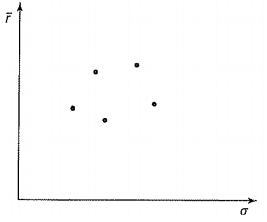
\includegraphics{images/First_Optimization_Photo.png}
\end{center}
\textbf{Variance Of A Portfolio: }Taking a portfolio of $X_1,\dots,X_n$ with weights $\omega_1,\dots,\omega_n$ and rate of return $r_1,\dots,r_n$ and covariances $\sigma_{ij}$. We can use this to calculate the total variance of the portfolio: 
\begin{align*}
    \sigma^2&=\text{Var}(\text{"Portfolio"})=\mathbb{E}\left[(r-\bar{r})^2\right]=\mathbb{E}\left[\left(\sum_{i=1}^n \omega_i r_i - \sum_{i=1}^n \omega_i \bar{r_i}\right)^2\right]= \\
     &= \mathbb{E}\left[\sum_{i=1}^n \omega_i\omega_j(r_i-\bar{r_i})(r_j-\bar{r_j})\right] = \sum_{i=1}^n\omega_i\omega_j \sigma_{ij}
\end{align*}
We will now return to the diagrams. Given 2 assets, we can look at the diagram and try to look at how the weighted sum $\alpha X_1+(1-\alpha)X_2$ appears in the diagram. The immediate problem we encounter is that the strict values in the diagram and $\alpha$ don't give the exact location of their weighted sum, since there is some influence of their covariance on the position of the weighted sum and this value doesn't appear in the diagram. But we can have some result (that we will not prove since the proof doesn't add much to the understanding of the topic, but it isn't all too complicated to prove): \\ \\
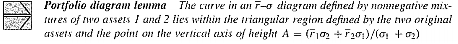
\includegraphics{images/Second_Optimization_Photo.png} \\
And this looks like: 
\begin{center}
    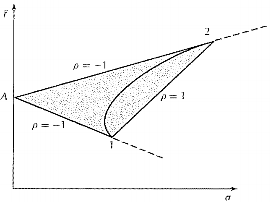
\includegraphics{images/Third_Optimization_Photo.png}    
\end{center}
Now we can do this for a portfolio (with more than 2 assets) with certain weights. What we are looking for is a weighted sum with a specific expected rate of return but with a minimized variance, looking at the diagram 
\begin{center}
    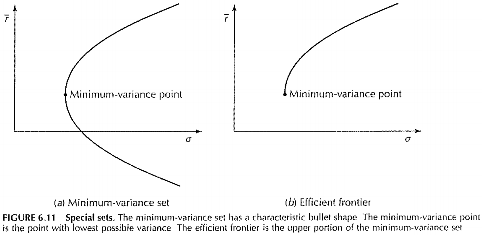
\includegraphics[scale=0.85]{images/Fourth_Optimization_Photo.png}
\end{center}
There will be a point with minimum variance for each expected rate of return (the set of points that are a minimum variance for some expected rate of return is called the efficient frontier) and so this begs the question - how to find this point for a specific expected rate of return? This problem is solved using the method that is called the Markowitz model.
The problem can be formulated using traditional optimization formatting in the following way - 
\begin{center}
    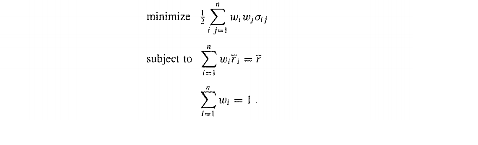
\includegraphics{images/Fifth_Optimization_Photo.png}    
\end{center}
The multiplication constant of $\frac{1}{2}$ is just for convenience sake and can be seen later. For the solution we will use the optimization concept of Lagrange Multipliers.\\\\
\subsection{Analytic Solution Of The Model}
First to do this we need to define exactly what functions we will use in the process - 
\[f(\omega_1,\dots,\omega_n) := \frac{1}{2}\sum_{i,j=1}^n \omega_i\omega_j\sigma_{ij}\]
with constraints
\begin{align*}
g_1(\omega_1,\dots,\omega_n) &:= \sum_{i=1}^n \omega_i \bar{r_i} -\bar{r} \\ g_2&:=\sum_{i=1}^n \omega_i - 1
\end{align*}
This tells us that the Lagrangian we need to define is - 
\begin{align*}
    \mathcal{L}(\omega_1,\dots,\omega_n,\lambda,\mu)&:= f(\omega_1\dots,\omega_n)-\lambda g_1(\omega_1,\dots,\omega_n)-\mu g_2(\omega_1,\dots,\omega_n)= \\
    &=\frac{1}{2}\sum_{i,j=1}^n \omega_i\omega_j\sigma_{ij} - \lambda\left(\sum_{i=1}^n \omega_i \bar{r_i} -\bar{r}\right) - \mu\left(\sum_{i=1}^n \omega_i - 1\right)
\end{align*}
Now we need to derive the Lagrangian according to each $\omega_i$ and compare to 0, and then compare the constraints to 0 to get a linear system that can be solved in a much easier fashion. Notice that for all of the above functions if we derive it according to $\omega_1$, then we can very quickly get the derivation according to each other $\omega_i$ because there is a very high degree of symmetry in the above functions. Therefore we will derive for $\omega_1$ and then generalize for each $\omega_i$. 
\[\frac{d\mathcal{L}}{d\omega_1} = \frac{df}{d\omega_1} - \lambda \frac{dg_1}{d\omega_1}-\mu\frac{dg_2}{f\omega_1}\]
Now notice that
\[\frac{df}{d\omega_1} = \left[\frac{1}{2}\sum_{i,j=1}^n \omega_i\omega_j\sigma_{ij}\right]_{\omega_1} = \frac{1}{2}\left(2\sum_{j=1}^n [\omega_1]_{\omega_1}\omega_j\sigma_{1j}\right) = \sum_{j=1}^n \omega_j\sigma_{1j}\]
\[\lambda\frac{dg_1}{d\omega_1}=\lambda\omega_1 r_1\]
\[\mu\frac{dg_2}{d\omega_1} = \mu\]
Putting all of this together we get
\[\frac{d\mathcal{L}}{d\omega_1} = \sum_{j=1}^n \omega_j \sigma_{1j} - \lambda \omega_1 r_1 - \mu\]
Now we can easily see that 
\[\frac{d\mathcal{L}}{d\omega_i} = \sum_{j=1}^n \omega_j \sigma_{ij} - \lambda \omega_i r_i - \mu\]
Putting all of this together we get the following n+2 linear equations with n+2 unknowns (which from the introduction we have that it should have a solution) whose solution is exactly what we are looking for - \begin{center}
    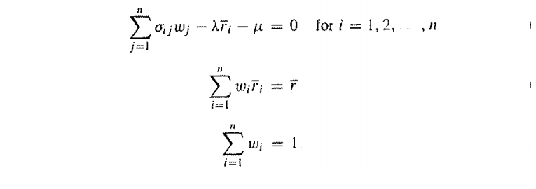
\includegraphics[scale=0.8]{images/Sixth_Optimization_Photo.png}    
\end{center}
\subsection{Implementation Of The Model On A Data Set}
We will now see an implementation of the model on the following given data from 10 periods of time:
\begin{table}[h!]
\centering
\begin{tabular}{||c c c c c c||} 
 \hline
   & Stock 1 & Stock 2 & Stock 3 & Stock 4 & Stock 5 \\ [0.5ex] 
 \hline\hline
 Period 1 & $10.00\%$ & $15.00\%$ & $12.00\%$ & $18.00\%$ & $5.00\%$ \\
 Period 2 & $12.00\%$ & $17.00\%$ & $13.00\%$ & $16.00\%$ & $8.00\%$ \\
 Period 3 & $8.00\%$ & $4.00\%$ & $9.00\%$ & $3.00\%$ & $10.00\%$ \\
 Period 4 & $7.00\%$ & $-8.00\%$ & $7.00\%$ & $4.00\%$ & $9.00\%$ \\
 Period 5 & $9.00\%$ & $15.00\%$ & $9.00\%$ & $8.00\%$ & $5.00\%$ \\ 
 Period 6 & $7.00\%$ & $22.00\%$ & $11.00\%$ & $10.00\%$ & $4.00\%$\\
 Period 7 & $8.00\%$ & $3.00\%$ & $9.00\%$ & $-3.00\%$ & $4.00\%$\\
 Period 8 & $6.00\%$ & $-14.00\%$ & $6.00\%$ & $15.00\%$ & $6.00\%$\\
 Period 9 & $9.00\%$ & $2.00\%$ & $8.00\%$ & $20.00\%$ & $8.00\%$\\
 Period 10 & $11.00\%$ & $15.00\%$ & $10.00\%$ & $16.00\%$ & $10.00\%$\\[1ex] 
 \hline
\end{tabular}
\caption{Historical data (returns) on stocks}
\end{table}\\
\textit{\textbf{Recall}: The expectation of a discrete random variable $X$ is defined as} \[\bar{X}=\mathbb{E}[X]=\sum_{x\in X}{x\cdot\mathbb{P}(X=x)}\] \textit{The variance of a random variable $X$ is defined as} \[\text{Var}(X):=\mathbb{E}[(X-\mathbb{E}[X])^2]=\mathbb{E}[X^2]-\mathbb{E}[X]^2\] \textit{and the covariance between two random variable $X, Y$ is defined as} \[\text{Cov}(X,Y):=\mathbb{E}[X Y]-\mathbb{E}[X]\mathbb{E}[Y]\]
Consider the uniform probability over the returns of our data. Our calculations were done as follows:
\begin{itemize}
    \item $\forall 1\le i \le 5: \bar{r}_i = \mathbb{E}[\text{"Stock i"}]=\frac{1}{10}\sum_{j = 1}^{10}{\text{[return of stock i in the j-th period]}}$
    \item $\forall 1\le i, j \le 5: \text{Cov}(\text{"Stock i", "Stock j"}) = \mathbb{E}[\text{"Stock i}\cdot\text{"Stock j"}]-\mathbb{E}[\text{"Stock i"}]\cdot \mathbb{E}[\text{"Stock j"}]= \frac{1}{100}\sum_{1\le l, k \le 10}[\text{return of stock i in the l-th period}]\cdot[\text{return of stock j in the k-th period}]-\bar{r}_i\bar{r}_j$
\end{itemize}
All the calculations were made with wolfram-alpha. (For the sake of the reader we did not include them in this paper.) We got that the expected return (mean value) vector for the five stocks is 
$$\bar{r}=\begin{pmatrix}
8.70\%\\
7.10\%\\
9.40\%\\
10.70\%\\
6.90\%
\end{pmatrix}$$
and the variance/covariance matrix of the five stocks is 
\begin{center}
    $\sigma=\begin{pmatrix}
    0.03\% & 0.12\% & 0.03\% & 0.06\% & 0.01\%\\
    0.12\% & 1.23\% & 0.20\% & 0.16\% & -0.05\%\\
    0.03\% & 0.20\% & 0.04\% & 0.04\% & -0.01\%\\
    0.06\% & 0.16\% & 0.04\% & 0.51\% & 0.02\%\\
    0.01\% & -0.05\% & -0.01\% & 0.02\% & 0.05\%
    \end{pmatrix}$
\end{center}
Our problem is to find a portfolio of the above stocks with an expected return of $8.56\%$ (this is the expected return for equal shares of the stocks, and it makes sense to find a solution for this value of return) which minimizes the risk, i.e., which has the optimal variance. Thus, our optimization problem is the following:
\begin{center}
    $\text{min }\frac{1}{2}\sum_{i, j =1}^{5}{\omega_i \omega_j \sigma_{i, j}}$\\
    $\text{s.t: } \sum_{i=1}^5{\omega_i\bar{r}_i} = 0.0856$\\
    $\sum_{i=1}^5{\omega_i}=1$
\end{center}
Using the Markowitz Model, we saw that a solution can be found using the Lagrange Multipliers optimization method. Therefore, we need to solve for 
$\omega_1, \omega_2, \omega_3, \omega_4, \omega_5, \lambda, \mu$ the following equations:
\begin{center}
$\begin{cases}
        0.0003\omega_1 +0.0012\omega_2 +0.0003\omega_3 +0.0006\omega_4 +0.0001\omega_5 -0.0870\lambda -\mu = 0\\
    0.0012\omega_1 +0.0123\omega_2 +0.0020\omega_3 +0.0016\omega_4 -0.0005\omega_5 -0.0710\lambda -\mu = 0\\
    0.0003\omega_1 +0.0020\omega_2 +0.0004\omega_3 +0.0004\omega_4 -0.0001\omega_5 -0.0940\lambda -\mu = 0\\
    0.0006\omega_1 +0.0016\omega_2 +0.0004\omega_3 +0.0051\omega_4 +0.0002\omega_5 -0.1070\lambda -\mu = 0\\
    0.0001\omega_1 -0.0005\omega_2 -0.0001\omega_3 +0.0002\omega_4 +0.0005\omega_5 -0.0690\lambda -\mu = 0\\
    0.0870\omega_1 +0.0710\omega_2 +0.0940\omega_3+0.1070\omega_4+0.0690\omega_5 = 0. 0856\\
    \omega_1+\omega_2+\omega_3+\omega_4+\omega_5 = 1
\end{cases}$
\end{center}
The first five equations can be solved linearly for $\omega_1, \omega_2, \omega_3, \omega_4, \omega_5$. We get:
\begin{center}
    $\begin{pmatrix}
    \omega_1\\ \omega_2\\ \omega_3\\ \omega_4\\ \omega_5
    \end{pmatrix} = \begin{pmatrix}
    (34194\lambda +355200\mu)/17 \\
    (3752\lambda +41600\mu)/51 \\
    (-85478\lambda -886400\mu)/51\\
    (-4490\lambda -50000\mu)/51\\
    (-8342\lambda -75600\mu)/17
    \end{pmatrix}$
\end{center}
Substitute the bottom two equations and solve for $\lambda, \mu$. (Again, we used wolfram-alpha to substitute and solve those two equations. For the sake of the reader, we did not include them in this paper.)\\
Our solution for optimal shares was:
\begin{center}
    $\begin{pmatrix}
    \omega_1\\ \omega_2\\ \omega_3\\ \omega_4\\ \omega_5
    \end{pmatrix} =\begin{pmatrix}
    2.51\% \\ 0.00\% \\ 64.59\% \\ 0.00\% \\ 32.90\%
    \end{pmatrix}$
\end{center}
which gave the optimal variance of $0.02\%$.
\end{document}
